\begin{tikzpicture}
\node[anchor=south west,inner sep=0] at (0,0) {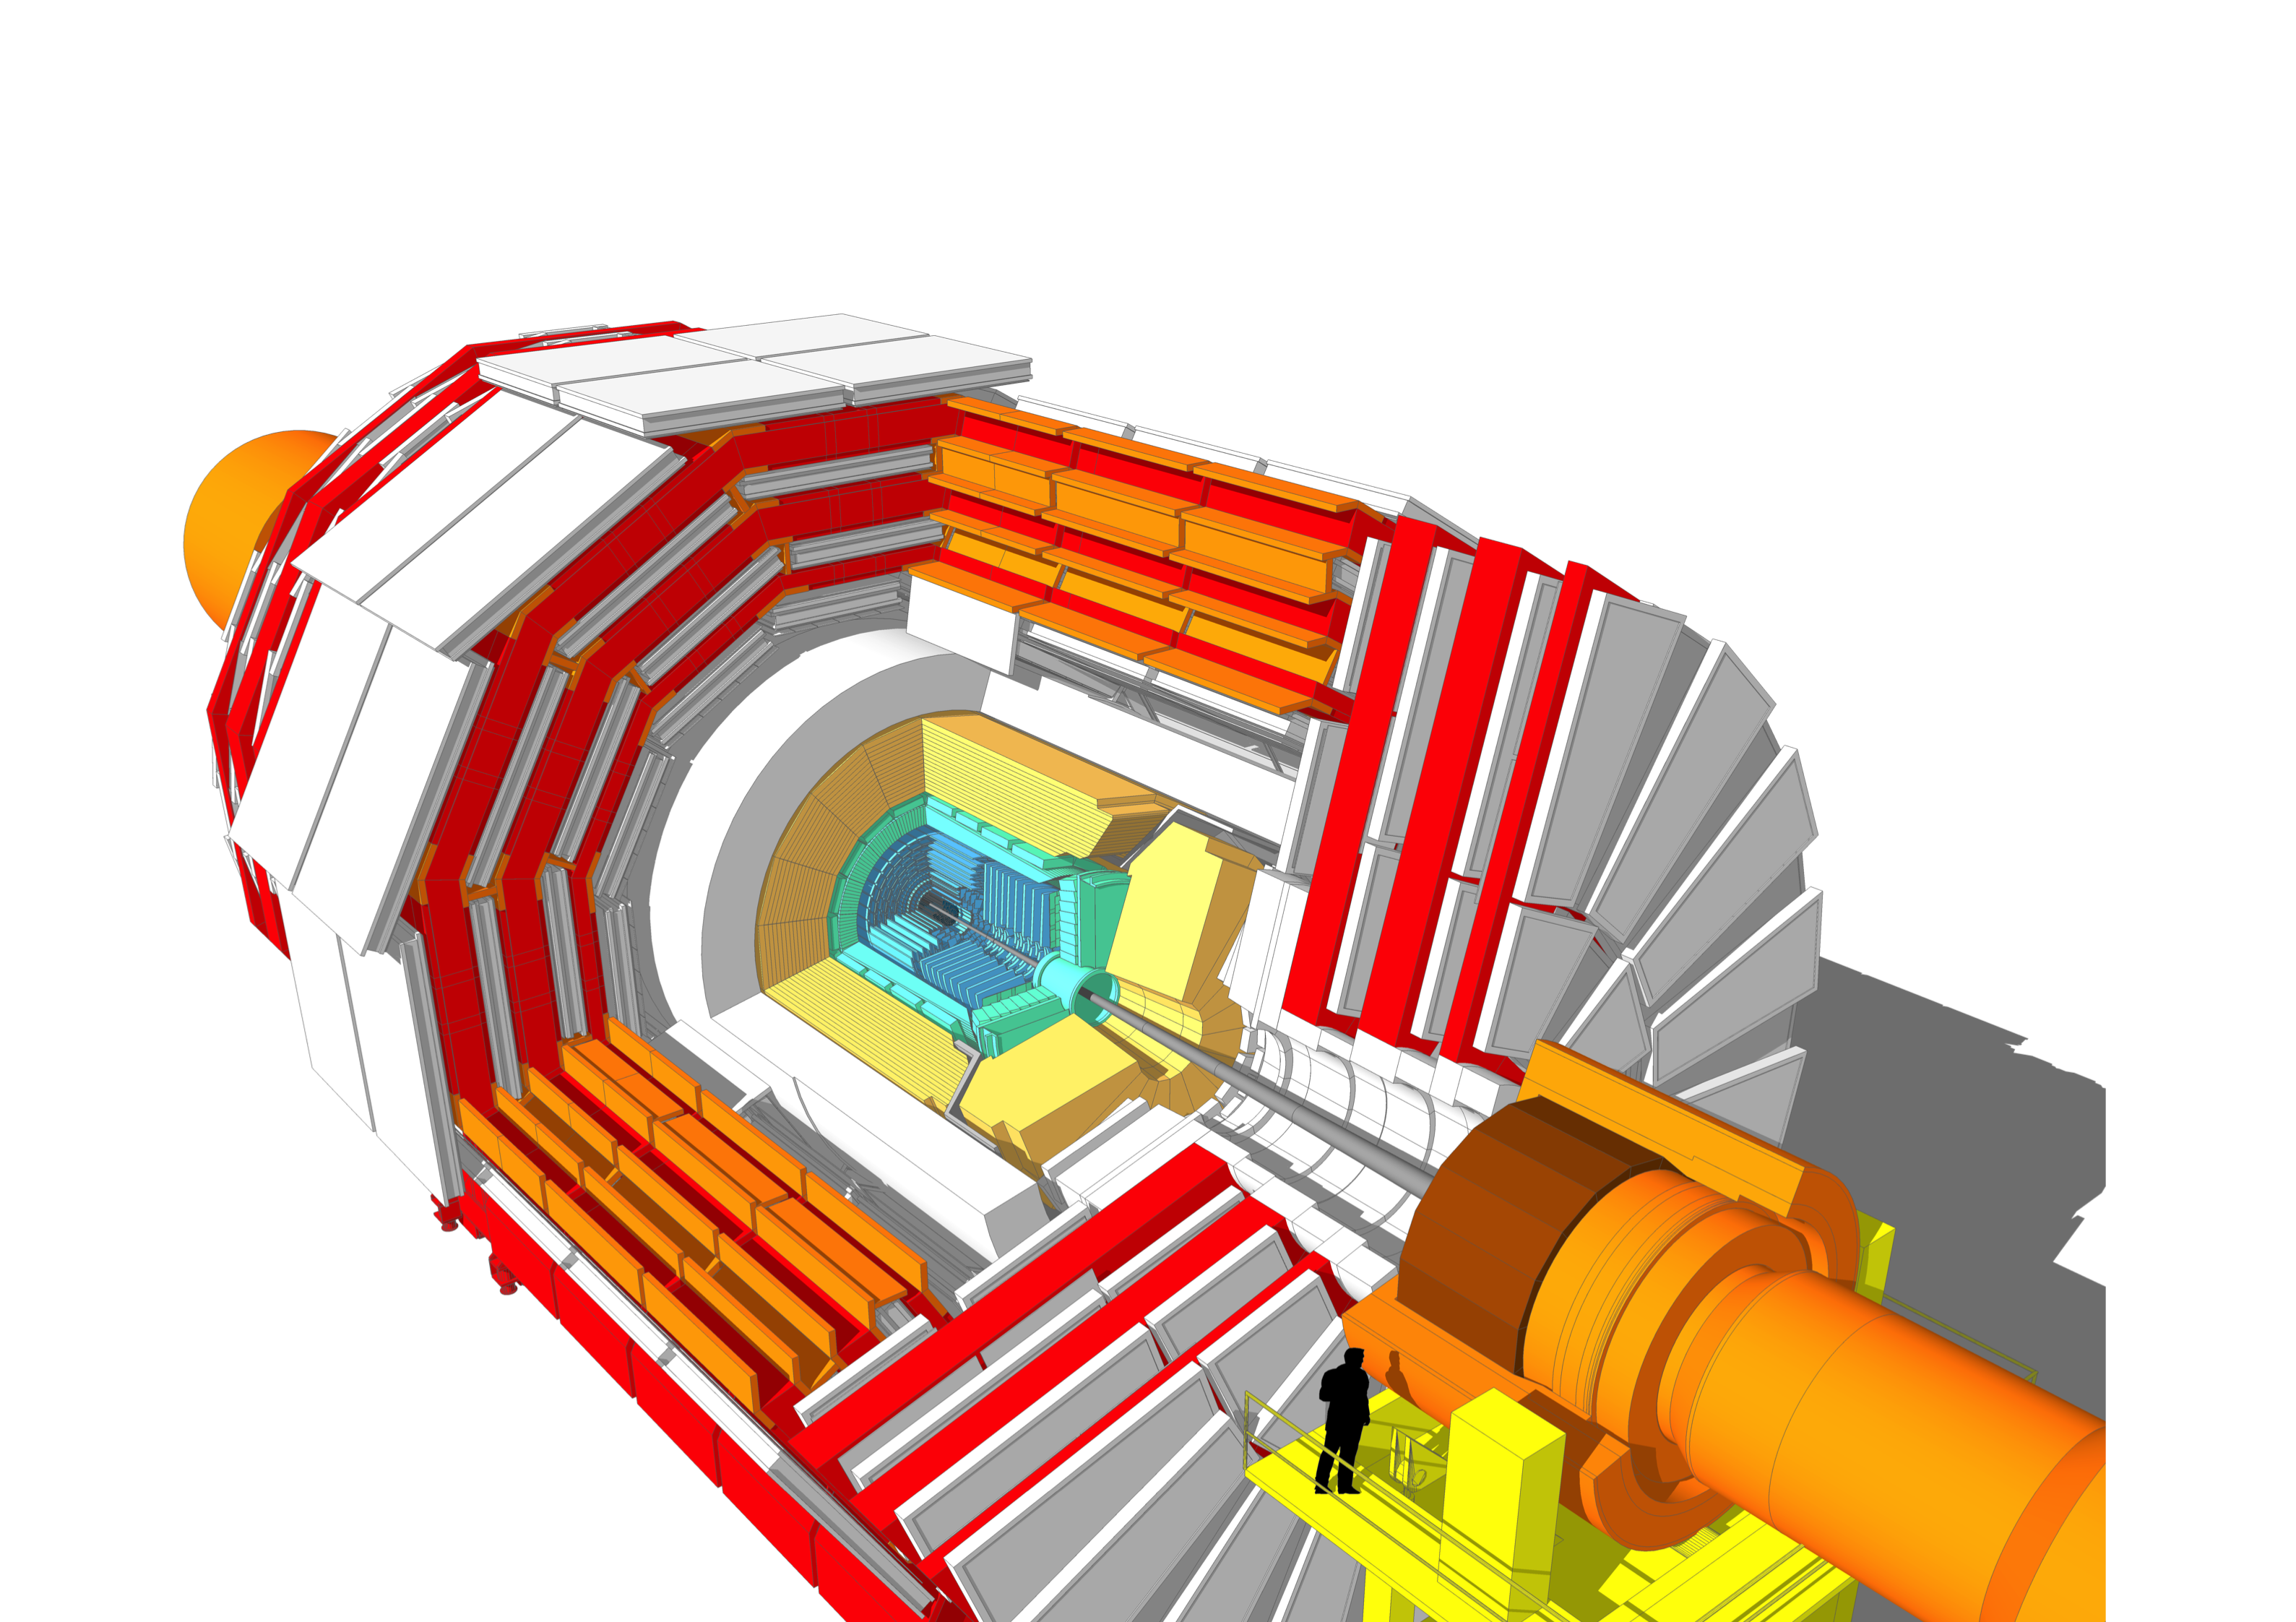
\includegraphics[width=17cm]{\PhDthesisdir/plots_and_images/CMS_slices/from_CMS_document_13631-v4/cms_160312_07.png}};
	
\draw (0.4, 11.55) node [right] {\small Détecteur CMS\vphantom{ÀQ}};

\draw (0.4, 11.05) node [right] {\tiny Masse totale\vphantom{ÀQ}};
\draw (0.4, 10.75) node [right] {\tiny Diamètre\vphantom{ÀQ}};
\draw (0.4, 10.45) node [right] {\tiny Longueur\vphantom{ÀQ}};
\draw (0.4, 10.15) node [right] {\tiny Champ magnétique\vphantom{ÀQ}};

\draw (2.3, 11.05) node [right] {\tiny : \num{14000} tonnes\vphantom{ÀQ}};
\draw (2.3, 10.75) node [right] {\tiny : \SI{15.0}{\meter}\vphantom{ÀQ}};
\draw (2.3, 10.45) node [right] {\tiny : \SI{28.7}{\meter}\vphantom{ÀQ}};
\draw (2.3, 10.15) node [right] {\tiny : \SI{3.8}{\tesla}\vphantom{ÀQ}};

\draw (4.7, 11.35) node [right] {\scriptsize Culasse de fer\vphantom{ÀQ}};
\draw (4.7, 11.05) node [right] {\tiny \num{12500} tonnes\vphantom{ÀQ}};

\draw (7.8, 11.05) node [right] {\scriptsize Trajectographe en silicium (\emph{tracker})\vphantom{ÀQ}};
\draw (7.8, 10.75) node [right] {\tiny Pixels ($\num{100}\times\SI{50}{\micro\meter^2})$  $\sim \SI{1.9}{\meter^2}$ $\sim \SI{124}{M}$ canaux\vphantom{ÀQ}};
\draw (7.8, 10.45) node [right] {\tiny Fils ($\num{80}-\SI{180}{\micro\meter}$) $\sim\SI{200}{\meter^2}$ $\sim\SI{9.6}{M}$ canaux\vphantom{ÀQ}};

\draw (10.2, 9.95) node [right] {\scriptsize Solénoïde supraconducteur\vphantom{ÀQ}};
\draw (10.2, 9.65) node [right] {\tiny Bobine de niobium-titane, courant de $\sim\SI{18000}{\ampere}$\vphantom{ÀQ}};

\draw (11.4, 9.00) node [right] {\scriptsize Chambres à muons\vphantom{ÀQ}};
\draw (11.4, 8.70) node [right] {\tiny Barillet : \num{250} tubes à dérive,\vphantom{ÀQ}};
\draw (11.4, 8.40) node [right] {\tiny \hphantom{Barillet :}\ \num{480} chambres à plaques résistives\vphantom{ÀQ}};
\draw (11.4, 8.10) node [right] {\tiny Bouchon : \num{540} chambres à pistes cathodiques,\vphantom{ÀQ}};
\draw (11.4, 7.80) node [right] {\tiny \hphantom{Bouchon :}\ \num{576} chambres à plaques résistives\vphantom{ÀQ}};

\draw (13.2, 7.10) node [right] {\scriptsize Détecteur de gerbes (PS)\vphantom{ÀQ}}; %Détecteur à pieds de gerbes
\draw (13.2, 6.80) node [right] {\tiny Fils de silicium $\sim\SI{16}{\meter^2}$\vphantom{ÀQ}};
\draw (13.2, 6.50) node [right] {\tiny \hphantom{Barillet :}\ $\sim\num{137000}$ canaux\vphantom{ÀQ}};

\draw (13.5, 5.80) node [right] {\scriptsize Calorimètre avancé (HF)\vphantom{ÀQ}};
\draw (13.5, 5.50) node [right] {\tiny Acier et fibres de quartz\vphantom{ÀQ}};
\draw (13.5, 5.20) node [right] {\tiny \hphantom{Barillet :}\ $\sim\num{2000}$ canaux\vphantom{ÀQ}};

\draw (0, 2.70) node [right] {\scriptsize Calorimètre\vphantom{ÀQ}};
\draw (0, 2.40) node [right] {\scriptsize électromagnétique (ECAL)\vphantom{ÀQ}};
\draw (0, 2.10) node [right] {\tiny $\sim\num{76000}$ cristaux de \ce{PbWO4}\vphantom{ÀQ}};

\draw (0.2, 0.85) node [right] {\scriptsize Calorimètre hadronique (HCAL)\vphantom{ÀQ}};
\draw (0.2, 0.55) node [right] {\tiny Laiton et plastique, $\sim\num{7000}$ canaux\vphantom{ÀQ}};

\foreach \startx/\starty/\endx/\endy in {
5.05/10.8/3.2/9,%
5.05/10.8/5.23/8.4,%
8.75/10.3/7.3/5.3,%
10.5/9.42/8.5/6.4,%
11.5/8.75/10.2/8.33,%
11.5/8.75/10.6/7.4,%
13.25/6.9/7.8/5.25,%
13.8/5.3/11.6/3.45,%
2/2.7/6.75/4.75,%
2/2.7/7.45/4.55,%
4.5/1/6.85/4.2,%
4.5/1/7.8/4.15}{
\draw (\startx, \starty) -- (\endx, \endy);
\fill (\endx, \endy) circle (2pt);
}

\end{tikzpicture}